
\section{The Road Module}
\label{sec:roadmodule}

The Road Module is the name given to the Python class present in the SML World that is responsible for all the functionalities related to the road network. Its functionalities can be divided into two broad scopes, the computation of car trajectories and the visualisation of the environment.

In this section, we will give an overview of the functionalities that the Road Module provides, and an explanation of it's internal algorithms, when necessary.

\subsection{Processing the Road Network Map}

The first task of the Road Module, is to process and make sense of the Road Network Map. To do so, the constructor of the class is provided with the \textit{.xml} file containing this information.

The constructor will parse the \textit{.xml}, and the class will store dictionaries for the existing nodes, ways and lanelets in said file. Additionally a dictionary storing all the found tags, and corresponding nodes, is also created.

\subsubsection{Converting from GPS to Meters}

As stated previously every OSM Node has an associated GPS latitude and longitude. For our purposes, we wish to have a simpler representation of the spatial location of the nodes, such as a Cartesian coordinate system in meters.

To do so we make use of the Python package \textbf{utm} (https://pypi.python.org/pypi/utm). This package allows us to make a conversion from GPS coordinates to a Cartesian referential as defined by the UTM convention. Once we have these new coordinates we will apply a translation transform so that they will be defined in a more convenient referential.

By default this new referential is located in the center of all the OSM Nodes. This center is computed easily by averaging the position of all the nodes. Once we know this center, we just need to subtract it from the coordinates of every single node, we will then have all of the node coordinates in the referential located in the center of all the nodes.

Another possibility is to define an Origin Node on which the referential will be located. To do so, when creating the \textit{.xml} file, one just need to and a node with the tag "origin"="true". If the Road Module detects that such a node is present in the file, it will simply subtract this node's Cartesian coordinates to all of the other nodes' coordinates, effectively making them be referenced on a referential located at the origin node.

\subsubsection{Computing Lanelet Adjacencies}

One of the most important parts of the road network is the adjacency between the lanelets, for it defines the possible ways that cars can drive in them.

To fully describe the adjacencies between lanelets, we will make use of an Adjacency Matrix. An adjacency matrix A, is a square matrix with $n \times n$ elements, where $n$ is the number of lanelets in the road network.

\[
A_{n,n} = 
 \begin{pmatrix}
  a_{1,1} & a_{1,2} & \cdots & a_{1,n} \\
  a_{2,1} & a_{2,2} & \cdots & a_{2,n} \\
  \vdots  & \vdots  & \ddots & \vdots  \\
  a_{n,1} & a_{n,2} & \cdots & a_{n,n} 
 \end{pmatrix}
\]
 
The entry $a_{i,j}$ in the matrix indicates the adjacency value between lanelet $i$ and lanelet $j$. If its is possible to go from lanelet $i$ and lanelet $j$, \textit{i.e.}, if it lanelet $i$ is adjacent to lanelet $j$, the value of $a_{i,j}$ will be equal to the length of lanelet $i$.

If the it is not possible to go from lanelet $i$ and lanelet $j$, the value of $a_{i,j}$ will be infinity, or an extremely large number (in the SML World implementation this value is $10^{10}$).

Notice that $a_{i,j}$ is not necessarily equal to $a_{j,i}$, as being able to go from lanelet $i$ to lanelet $j$, does not imply that it is possible to go from lanelet $j$ to lanelet $i$.

\subsection{Computing Car Paths}

Computing a car path is equivalent to finding a valid/feasible way of going from one point in the road network to another. To do so, we divide this process in several parts.

\subsubsection{The Start and End Nodes of the Path}

The main inputs to the Path Finding algorithm are the Start Node and the End Node. The start and the end nodes define, respectively, where we wish our path to start, and where we want it to end.

Given the start node, the Road Module will find the lanelet (or lanelets) that have this node in as part of their right\_lane\_marking way. For now lets assume that only one lanelet contains this node. The same is done for the end node, and the lanelet containing it is found. We now have two lanelets that we will call $lanelet_{start}$ and $lanelet_{end}$, which contain the start and end node, respectively.

We now have a way to move from $lanelet_{start}$ to $lanelet_{end}$. The solution to this problem will be a path of lanelets, that will start in $lanelet_{start}$ and finish in $lanelet_{end}$, making only legal movements, \textit{i.e.}, transitions between adjacent lanelets.

\subsubsection{The Dijkstra Algorithm}

We wish to go from the starting lanelet to the ending lanelet, making transitions only between lanelets that are adjacent. We also want to do it in the best way possible, \textit{i.e.}, shortest way possible. 

This problem can be easily solved using the well known Dijkstra Algorithm. The Dijkstra algorithm is able to find the shortest path between nodes in a graph. We can view our road network as a graph of lanelets, in fact, the Lanelet Adjacency Matrix, perfectly defines a graph, where the lanelets are the nodes of the graph, and the edges are defined by the weights given by the adjacency matrix elements. An element of the matrix with an infinite value is equivalent to a non-existing edge.

This means, that having $lanelet_{start}$, $lanelet_{end}$, and the lanelet adjacency matrix, we can run the Dijkstra algorithm, and find the shortest path of lanelets between $lanelet_{start}$ and $lanelet_{end}$.

\subsubsection{Generating the Path}

Assume now, that after our Dijkstra algorithm, we found a solution path $ [lanelet_{start},\allowbreak lanelet_{a},\allowbreak lanelet_{b},\allowbreak lanelet_{c},\allowbreak lanelet_{end}]$. We now wish to get the $(x,y)$ path corresponding to this lanelet path. 

The $(x,y)$ path of a lanelet, which is the set of points centred between the left\_lane\_marking and right\_lane\_marking, where each point is equally distant to the next and previous points.

We compute the $(x,y)$ path for each lanelet in the lanelet path, stitch them together, forming an $(x,y)$ from $lanelet_{start}$ to $lanelet_{end}$ that complies with the rules of the road network (as defined in the lanelet adjacency matrix).

This path still needs a final modification, however. The path is made up of the full $(x,y)$ paths of each lanelet, including the $lanelet_{start}$ and $lanelet_{end}$, however we might not need the full path of the $lanelet_{start}$ and $lanelet_{end}$. Take for example the case where the prvided ending node is located somewhere in the middle of $lanelet_{end}$. In this case we will not want the full $(x,y)$ path of the lanelet, but only the section that starts at the beginning of the lanelet, and ends close to he ending node. The same principle applies to the $(x,y)$ path of $lanelet_{start}$, however resulting path will begin at the starting node and continue until the end of the lanelet. We call this procedure, cropping the trajectory.

\subsubsection{The "Circular" Dijkstra Algorithm}

The "Circular" Dijkstra algorithm is a special situation of the Dijkstra algorithm, in which we wish to find the shortest way from a node to itself, whilst assuming that nodes cannot connect to themselves. The importance of this algorithm for the SML World, has to do with generating paths that loop, thus resulting in motions that can run forever.

The original previous formulation of the Dijkstra algorithm does not allow us to solve this problem, however a simple reformulation can be done, that will allow us to find the shortest path from a node to itself.

To solve this problem we will need to create a new graph, that will be equivalent to the original graph, but that will allow us to solve the problem. Given that we want to find the shortest path from $node_i$ to itself, we will have to replace $node_i$ by nodes $node_i^{start}$ and $node_i^{end}$. $node_i^{start}$ will have all of the outgoing edges of $node_i$, and $node_i^{end}$ will have an of the incoming edges of $node_i$. 

Once this new graph is defined we can simply run a Dijkstra algorithm to find the shortest path between $node_i^{start}$ and $node_i^{end}$, and this will be equivalent to the shortest path from $node_i$ to itself.

\subsection{Environment Visualisation}

Besides defining how the road network behaves, the Road Module is also responsible for how the environment looks like. This is an important task as the visualisation of the environment plays a big role in the SML World.

Generating and visualising the environment requires the use of the graphical library pygame. More information about pygame can be found in their website \cite{pygame}.

\subsubsection{Drawing Patterns}

The first step consists in generating the environment background. For this purpose we start by repeating the pattern image that we wish to fill the background with. Usually we use a forest pattern as can be seen in figure \ref{fig:visualisation_background}. The forest pattern is simply applied through the whole image, as it is a background pattern. One can choose different any possible background by selecting the appropriate image pattern.

\begin{figure}[h!]
  \centering
    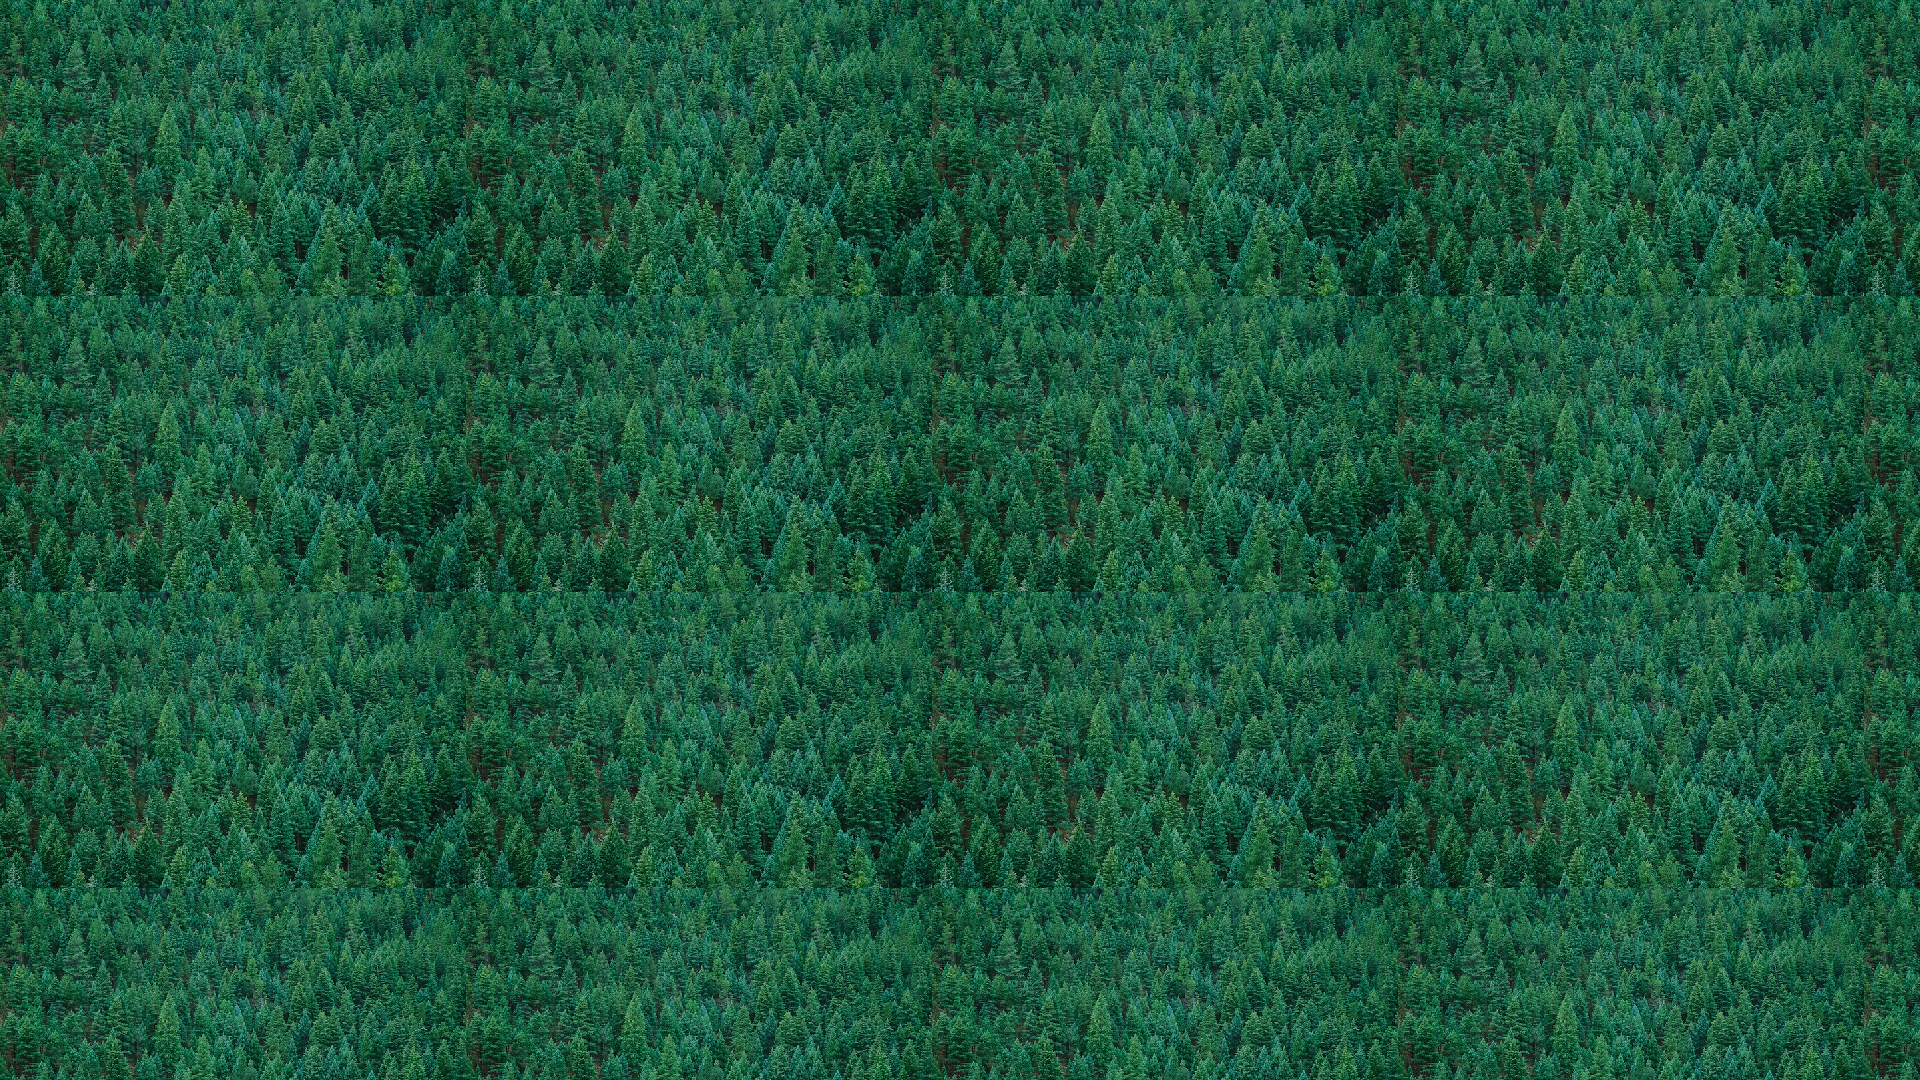
\includegraphics[width=0.95\textwidth]{visualisation_background}
    \caption{An environment with a forest pattern as background \label{fig:visualisation_background} }
\end{figure}

Once the background is drawn, we will overlay it with the roads. The roads are simply drawn by repeating a road pattern in the pixels corresponding to lanelets. First we find the regions of the lanelets, also called a mask. This mask tells us all the pixels that correspond to lanelets. Once we know this mask, we know where the lanelets are. We use this information to repeat the road pattern in the regions where there are lanelets. The result is shown in figure \ref{fig:visualisation_background_and_roads}. We can choose different looks for the roads by simply selecting the appropriate pattern image. 

\begin{figure}[h!]
  \centering
    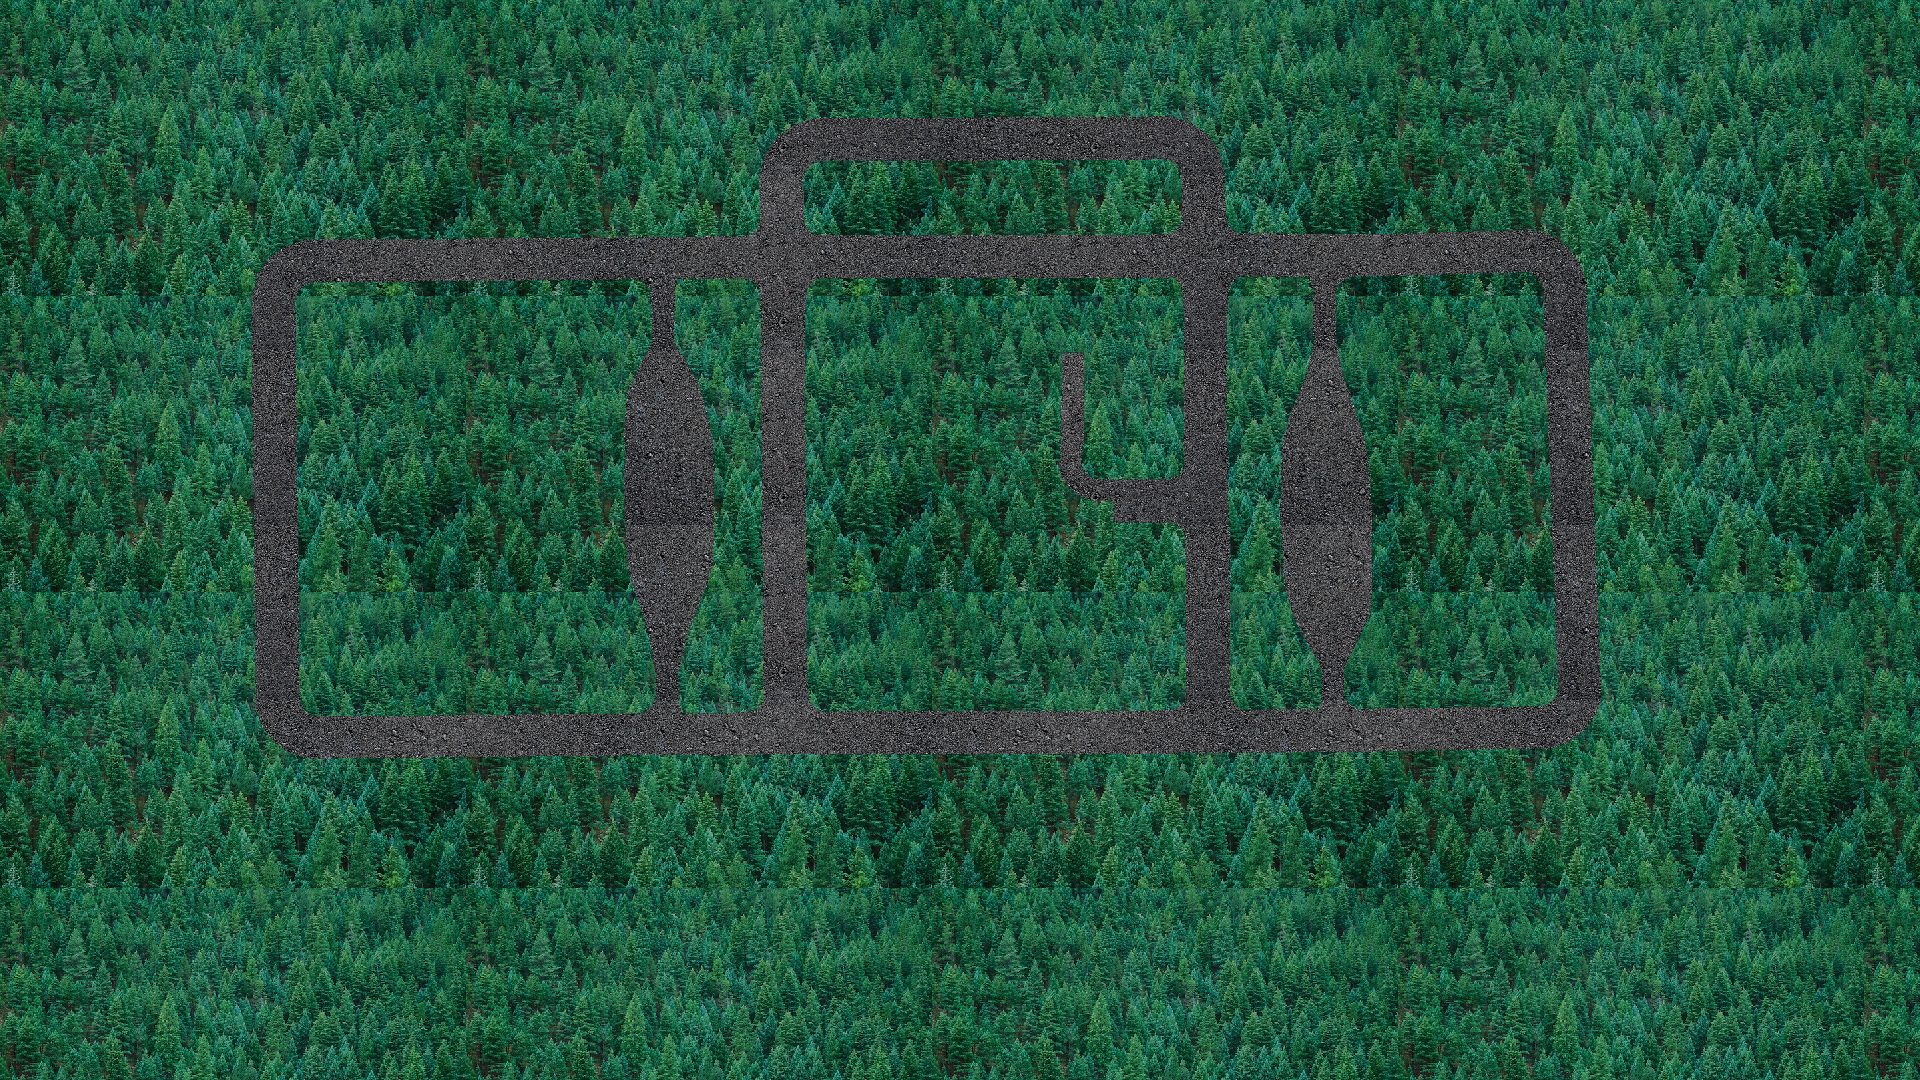
\includegraphics[width=0.95\textwidth]{visualisation_background_and_roads}
    \caption{An environment with a road pattern added \label{fig:visualisation_background_and_roads} }
\end{figure}

The environment visualisation can be made arbitrarily complex, if one uses this pattern repeat functionality to draw several different regions of different types. Figure \ref{fig:visualisation_background_with_several_patterns} shows an environment using five different patterns: forest, road, mud, iron and parking lot.

\begin{figure}[h!]
  \centering
    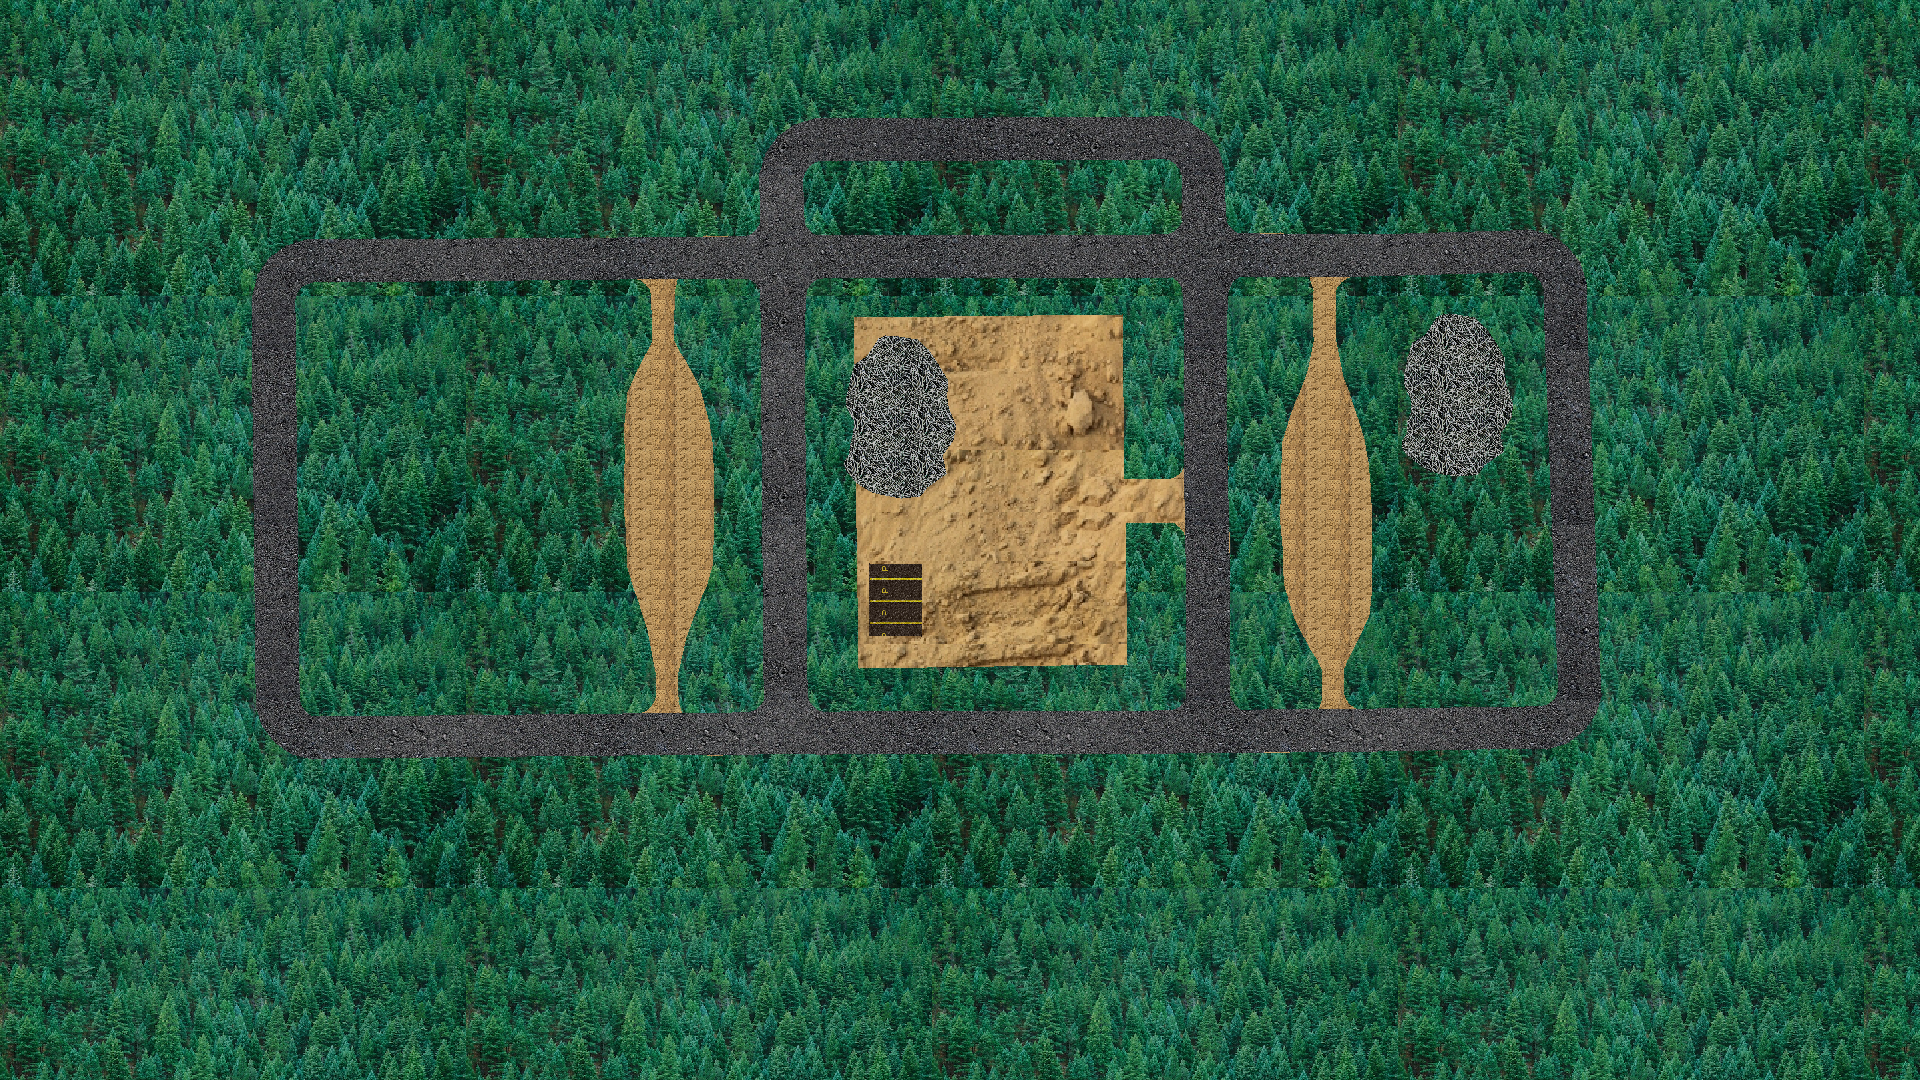
\includegraphics[width=0.95\textwidth]{visualisation_background_with_several_patterns}
    \caption{An environment using several patterns \label{fig:visualisation_background_with_several_patterns} }
\end{figure}

\subsubsection{Drawing Lines}

Another important part of the environment visualisation is the ability to draw lines. Drawing lines comes in handy when drawing road markings. The road module is able to draw lines of different colors and different widths for ways that are present in the road network, this can be seen in figure \ref{fig:visualisation_background_and_roads_and_markings}. The road module will go over all of the ways present in the road network and it will draw lines on top of them if they have a specific tag. In case they have a tag "line\_type"="interior", they will be drawn as a white line, if the tag is "line\_type"="exterior" they will be drawn as yellow lines. If a way has no tag, a line is not drawn. 

\begin{figure}[h!]
  \centering
    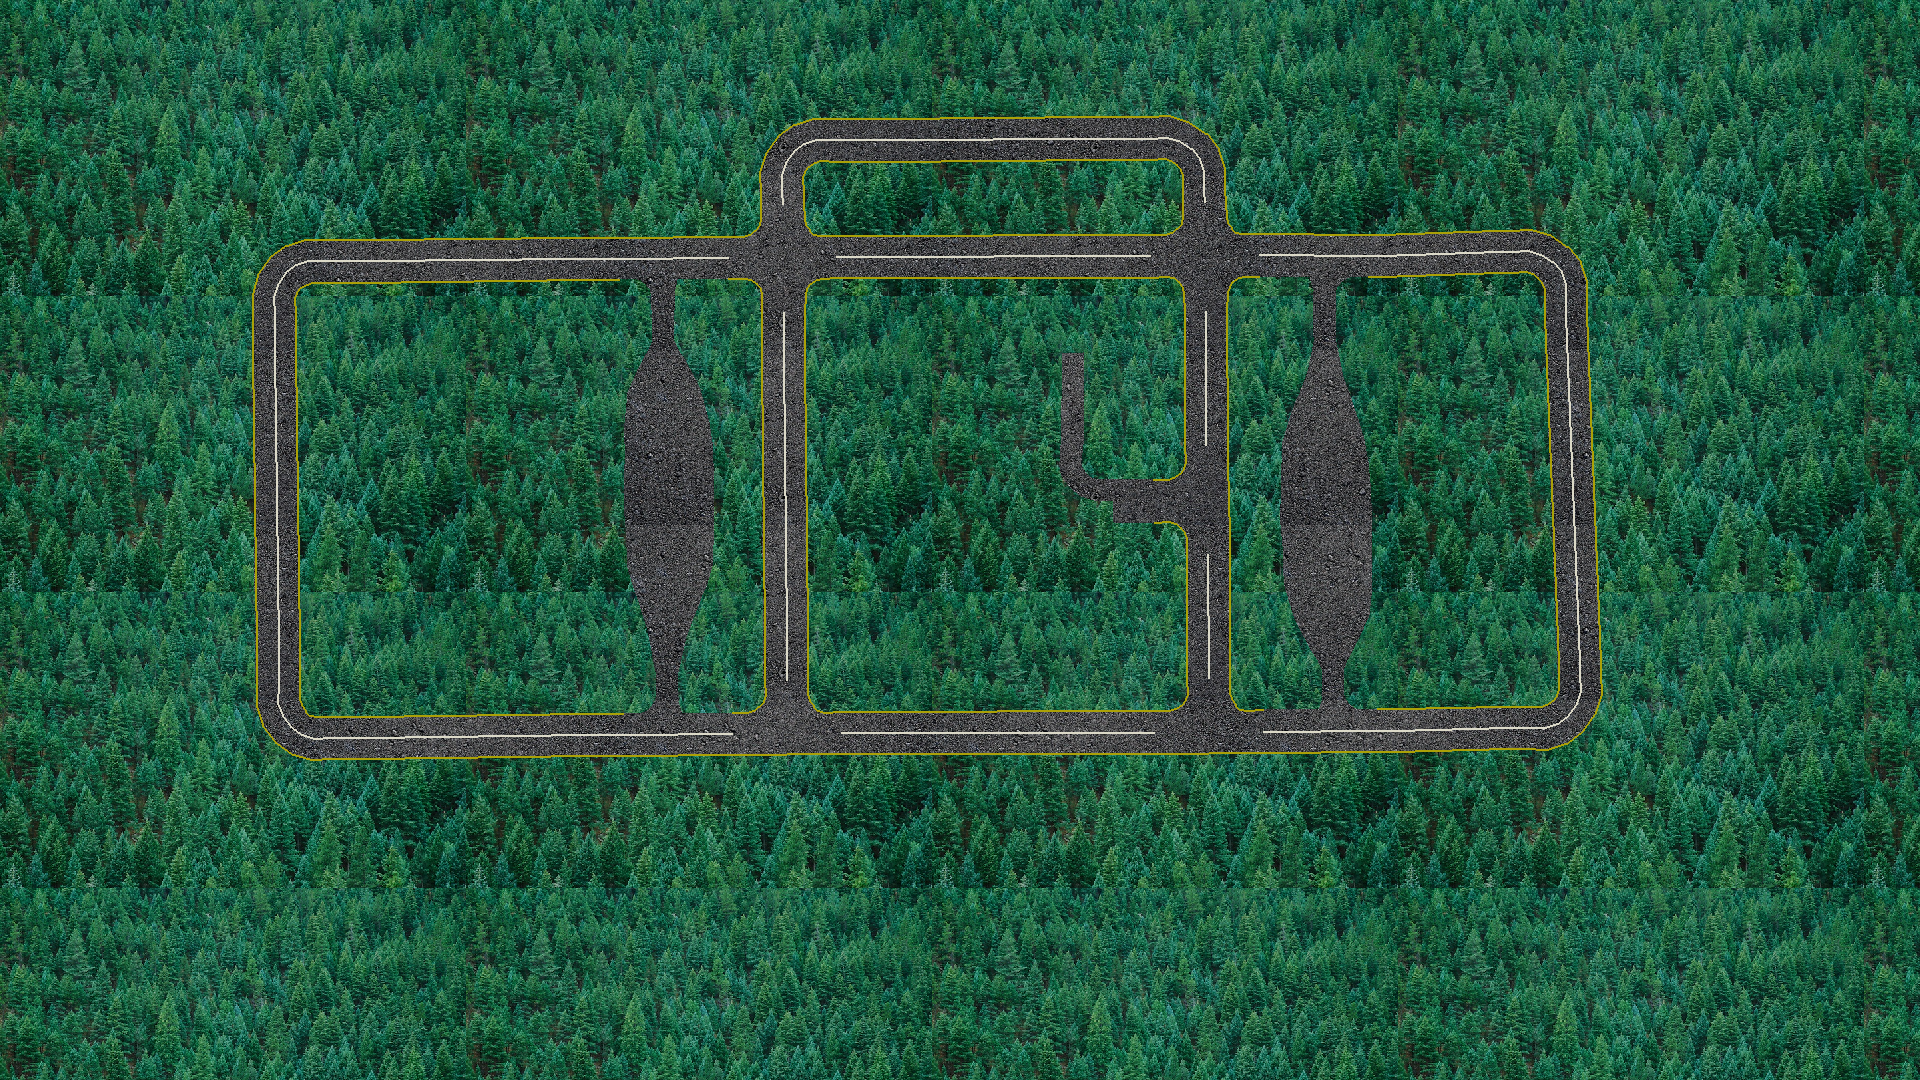
\includegraphics[width=0.95\textwidth]{visualisation_background_and_roads_and_markings}
    \caption{An environment with lines drawn \label{fig:visualisation_background_and_roads_and_markings} }
\end{figure}

\subsection{Using the Road Module}

Here we will briefly explain the main usages of the Road Module from a programming point of view. More detailed information is available in the source code.


\subsubsection{RoadModule()}

road\_module = RoadModule(xml\_file\_location) Constructs an instance of the class \texttt{RoadModule}. The constructor requires that the location of the \textit{.xml} defining the road network is given.

\subsubsection{SetImageProperties()}

SetImageProperties sets the properties of the image that will correspond to the environment. As arguments ImageWidth and ImageHeight correspond to the desired image width and height in pixels. PixelPerMeter will define how many pixels correspond to a meter in the map. Decreasing the value of PixelPerMeter will make the image correspond to a larger environment area.

\subsubsection{GetEnvironmentImage()}

GetEnvironmentImage generates and returns the image of the enviroment. The arguments required are the same as the ones in SetImageProperties. This method returns a pygame Surface corresponding to the environment image.

\subsubsection{GetPathBetweenNodeIds()}

GetPathBetweenNodeIds returns an $(x,y)$ path between two nodes. The arguments are StartOsmNodeId and EndOsmNodeId, which correspond to the ids of the nodes we wish that define this path. The third argument is PointsPerMeter wich indicates how many path points will be generated for each meter of path.

\subsubsection{GetPathBetweenNodeTags()}

Equivalent to GetPathBetweenNodeIds, however instead of having node ids as arguments, we have node tags. This allows for a simpler usage, as it is usually easier to know the tag of a node (it can be easily added on the road network \textit{.xml} file), than its id.

\subsubsection{GetClosedPathFromNodeId()}

Returns the $(x,y)$ path that starting and ending on a given node. The arguments are OsmNodeId and PointsPerMeter. OsmNodeId corresponds to the id of the node we wish to have the circular path of. PointsPerMeter will define how many path points will be generated for each meter of path.

\subsubsection{GetClosedPathFromNodeTag()}

Equivalent to GetClosedPathFromNodeId, however istead of providing a node id, the user provides a node tag.

\subsection{Deprecated Functionalities}

